\documentclass{article}\usepackage[]{graphicx}\usepackage[]{color}
%% maxwidth is the original width if it is less than linewidth
%% otherwise use linewidth (to make sure the graphics do not exceed the margin)
\makeatletter
\def\maxwidth{ %
  \ifdim\Gin@nat@width>\linewidth
    \linewidth
  \else
    \Gin@nat@width
  \fi
}
\makeatother

\definecolor{fgcolor}{rgb}{0.345, 0.345, 0.345}
\newcommand{\hlnum}[1]{\textcolor[rgb]{0.686,0.059,0.569}{#1}}%
\newcommand{\hlstr}[1]{\textcolor[rgb]{0.192,0.494,0.8}{#1}}%
\newcommand{\hlcom}[1]{\textcolor[rgb]{0.678,0.584,0.686}{\textit{#1}}}%
\newcommand{\hlopt}[1]{\textcolor[rgb]{0,0,0}{#1}}%
\newcommand{\hlstd}[1]{\textcolor[rgb]{0.345,0.345,0.345}{#1}}%
\newcommand{\hlkwa}[1]{\textcolor[rgb]{0.161,0.373,0.58}{\textbf{#1}}}%
\newcommand{\hlkwb}[1]{\textcolor[rgb]{0.69,0.353,0.396}{#1}}%
\newcommand{\hlkwc}[1]{\textcolor[rgb]{0.333,0.667,0.333}{#1}}%
\newcommand{\hlkwd}[1]{\textcolor[rgb]{0.737,0.353,0.396}{\textbf{#1}}}%
\let\hlipl\hlkwb

\usepackage{framed}
\makeatletter
\newenvironment{kframe}{%
 \def\at@end@of@kframe{}%
 \ifinner\ifhmode%
  \def\at@end@of@kframe{\end{minipage}}%
  \begin{minipage}{\columnwidth}%
 \fi\fi%
 \def\FrameCommand##1{\hskip\@totalleftmargin \hskip-\fboxsep
 \colorbox{shadecolor}{##1}\hskip-\fboxsep
     % There is no \\@totalrightmargin, so:
     \hskip-\linewidth \hskip-\@totalleftmargin \hskip\columnwidth}%
 \MakeFramed {\advance\hsize-\width
   \@totalleftmargin\z@ \linewidth\hsize
   \@setminipage}}%
 {\par\unskip\endMakeFramed%
 \at@end@of@kframe}
\makeatother

\definecolor{shadecolor}{rgb}{.97, .97, .97}
\definecolor{messagecolor}{rgb}{0, 0, 0}
\definecolor{warningcolor}{rgb}{1, 0, 1}
\definecolor{errorcolor}{rgb}{1, 0, 0}
\newenvironment{knitrout}{}{} % an empty environment to be redefined in TeX

\usepackage{alltt}
\title{Stat159: College. Where should I apply? \\ An interactive app to help at-risk students decide}
\author{Liang Hao, Bret Hart, Andrew Shibata, Gary Nguyen}
\date{\today}

\usepackage{hyperref}
\IfFileExists{upquote.sty}{\usepackage{upquote}}{}
\begin{document}

\maketitle
\section{Abstract}

This project carries out extensive analysis on the publicly available College Scorecard dataset, a huge database of detailed information on almost every single college in the United States, spanning back decades. The main output of this analysis is a working, interactive, dynamically responsive Shiny App that can be used by students to suggest schools appropriate to their needs. Of particular moral interest to our mission is serving minority, first-generation, at-risk students - thus, the responses are modeled around one basic tenet: a high-quality, low-cost education that will best uniquely serve the student that truly needs it.


\maketitle
\section{Introduction}

We are assuming the role of consultants to an NGO which primarily desires to provide at-risk, low-income, minority students a portfolio of colleges which best serve their needs: a high-quality, low-cost education. The interactive final product which allows student input is the shiny tool. Students enter in various criteria (their GPA, location, desired field of study, income bracket, first-generation status, etc) and it outputs a list of colleges ranked according to a score which we arbitrarily, but intelligently create as an ad-hoc indicator of "quality" of school for varying types of students. The responses are sorted upon this composite metric of "quality," and are readjusted in real time if the student changes their inputs. This "college quality score" is our response variable that students see and interact with, and the method the output list of schools are sorted upon.\newline

The actual disparate pieces of the response score are included as a result of a variety of exploratory analyses. At first, we underwent the daunting task of reading through the Data Dictionary given with the College Scorecard data - a detailed account of the content of around 2000 columns. After we became familiar with the general structure and material within the dataset, we moved on to research and exploratory data analysis. While there is some interesting philosophical merit to deliberating upon what makes a school "good," the definition of "good" we adopted allowed for a much more supervised process of creating a response variable - the majority of emphasis was placed on cost, community, and projections of success after college. Thus, we carried out research on relevant statistical literature. By looking through the data dictionary and reading some analytical publications that used the College Scorecard dataset, we began to put together a set of salient quality indicators, such as average salary after college, completion rate, median debt, or net price relative to a student's income bracket. \href{http://bit.ly/2gGW2fG}{This piece, especially from page 7 on, was of huge help to finalizing and legitimating this performance metric.}\newline

We then combine these responses into one "college quality score" for the school, with weights for different variables in the composite metric based upon experimentation and what the literature suggests. Additionally, We use combined data from the last 5 years for our score to reduce variance, with each year prior given less weight. The interesting specificity of our model is that it is geared not toward creating a score for general school quality and a prediction for the average student, but specifically for helping at-risk students who need assistance in deciding which schools are worth the application in their specific circumstances. These students truthfully and historically have not gotten the help that they deserve and we want to accommodate them.

\maketitle
\section{Data}



\subsection{Description}

The data used in the construction of this app originates from the \emph{College Scorecard} database, which is developed by the U.S. Department of Education (under Obama's Administration) to provide "key indicators about the cost and value of institutions across the country to help students choose a school that is well-suited to meet their needs, priced affordably, and is consistent with their educational and career goals." The dataset can be accessed  \href{https://collegescorecard.ed.gov/data/}{here}.

\subsection{Cleaning}
For our purpose, we interpret and intercalate the data from the past five years, cleaning and merging the sets by implementing the following algorithm:\newline

1: For each dataset, we extract the columns and rows with less than 10\% \emph{PrivacySuppressed} or \emph{NaN} to obtain usable datasets with each column posessing enough information to be meaningful. We then take the unions and overlaps of the columns and rows across the years. This leaves us with around 600 columns and 6700 colleges.\newline


2: We examine the data dictionary and relevant literature, noting useful columns that may be relevant to our response variable. This arbitrarion process decreases the number of columns to under 300. We then parse the five datasets with the logically collected columns and rows.\newline

3: While we include five years of data to ease out short-term variances, we still believe more recent data has value in this circumstance, so we combine the five datasets with the following weights:

\begin{table}[ht]
\centering
\begin{tabular}{rrrrrr}
  \hline
 & Year 14-15 & Year 13-14 & Year 12-13 & Year 11-12 & Year 10-11 \\ 
  \hline
Weight & 0.40 & 0.30 & 0.10 & 0.05 & 0.05 \\ 
   \hline
\end{tabular}
\end{table}


4: Lastly, we merge the combined dataset with the \emph{Post-Graduation Salary} dataset, which contains various variables not included in the original database (despite its insane size) to form the data frame used in this project. 

\subsection{Exploratory Data Analysis}

\subsubsection{Geographical Distribution}
To gain a better sense of what we want students to input or what we should include as an important piece in the response metric, We carry out substantial exploratory data analysis. We begin by looking at colleges around the country as a whole.\newline

First, let's look at the geographical distribution of colleges in the dataset. (For the purpose of efficient  and realistic graphing, the plot unfortunately only shows colleges present in the mainland United States.

\begin{knitrout}
\definecolor{shadecolor}{rgb}{0.969, 0.969, 0.969}\color{fgcolor}

{\centering 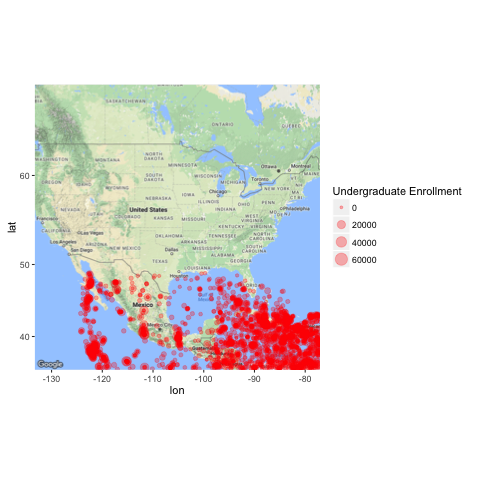
\includegraphics[width=300px]{../images/ggmap-schoolDistribution} 

}



\end{knitrout}

We see that there are a good number of schools of substantial size in most states, with the mid-western, mountain hemisphere perhaps a little low on number of educational institutions.\newline

Then, we may look at the "difficulty" of schools around the country, that is, the rejection rates, from 0\% to 100\%. 

\begin{knitrout}
\definecolor{shadecolor}{rgb}{0.969, 0.969, 0.969}\color{fgcolor}

{\centering 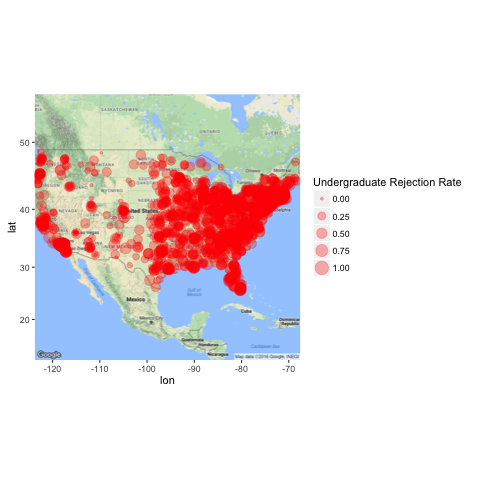
\includegraphics[width=300px]{../images/ggmap-admissionRateDistribution} 

}



\end{knitrout}

It's hard to tell as the points are smaller for lower acceptance rates, but there honestly doesn't seem to be a deficiency anywhere in schools that are, perhaps, easier to get in to, but which will undoubtedly provide a good education - this is exactly what we wanted to know. Is it even worth it to work on this recommendation platform at all? Yes, because students may have schools in their own backyards that they just need to be told about to explore and succeed. 

\subsubsection{Ethnicity}

It is no secret that those of minority racial/ethnic status in the United States may not be given the same institutional affordances in the college process, from admissions to graduation to post-graduation achievement. Even beyond negative and arbitrary admissions processes, it has been theorized that the existence of a community which is composed of students of your background, etc. can have a profound effect on success. Thus, we can examine the various ways race has been historicized in the college process, as it is and always will be of great public concern. Additionally, due to our NGO affiliation, we want to approach these institutional inequalities with a constructive open mind and a tool which suggests schools of better, or at least matching, diversity. 


\begin{table}[ht]
\centering
\begin{tabular}{rlll}
  \hline
 & Flag & Count & RelativeFrequency \\ 
  \hline
1 & Non Historically Black & 6613 & 0.985 \\ 
  2 & Historically Black & 102 & 0.015 \\ 
  3 & Non Predominantly Black & 6622 & 0.986 \\ 
  4 & Predominantly Black & 93 & 0.014 \\ 
  5 & Non Alaska Native Hawaiian serving & 6680 & 0.995 \\ 
  6 & Alaska Native Hawaiian serving & 35 & 0.005 \\ 
  7 & Non Tribal & 6684 & 0.995 \\ 
  8 & Tribal & 31 & 0.005 \\ 
  9 & Non Asian American Native American Pacific Islander & 6586 & 0.981 \\ 
  10 & Asian American Native American Pacific Islander & 129 & 0.019 \\ 
  11 & Non Hispanic & 6368 & 0.948 \\ 
  12 & Hispanic & 347 & 0.052 \\ 
   \hline
\end{tabular}
\caption{Flag for Historically Minority Serving Institute} 
\end{table}


From these tables, we gathered that minority groups are underrepresented in the vast majority of institutions, and thus, these students may feel out of place in an environment that is mostly made up of people different than them. As a contrast to these damning tables, we offer a simple pie chart which shows racial/ethnic demographics across the schools.

\begin{knitrout}
\definecolor{shadecolor}{rgb}{0.969, 0.969, 0.969}\color{fgcolor}

{\centering 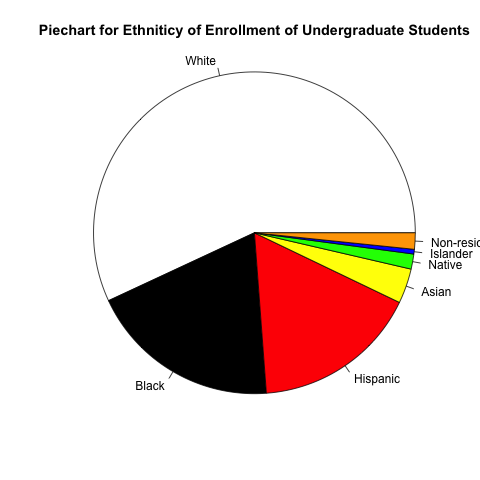
\includegraphics[width=250px]{../images/piechart-enrollmentEthnicity} 

}



\end{knitrout}

From the pie chart above, we may see that, while it is of course a problematic and contentious postulation, that white students make up the largest majority of the student body - thus, our metric of predominance in an institution may be unrealistic or not the greatest actual marker of diversity. 

\subsubsection{Net Price}
Net price is the final cost of attending an institution, which includes the amount required for tuition and fees, books and supplies, and living expenses after financial aid which would be on-default given to certain income levels. Thus, the Net Price is different for each income bracket - and our model reflects this, by pulling from different columns for net price in response to the student's input. For this project, we are obviously interested in the Average Net Price for full-time, first-time undergraduate Title IV-receiving students.\newline

Average net price $(NPT4 *$ for $PUB$ [public colleges; for public institutions, this metric is limited to those undergraduates who pay in-state tuition] and $PRIV$ [private colleges]) contains a weighted average of the net cost of attendance for all full-time, first-time undergraduate Title IV-receiving students.\newline

Here, summary statistics are provided for both Private and Public Institutions.\newline

\begin{table}[ht]
\centering
\begin{tabular}{rrrrrrrrrr}
  \hline
 & Min. & Max. & Range & Median & 25th & 75th & IQR & Mean & SD \\ 
  \hline
Public & 126.32 & 27055.80 & 26929.48 & 8604.50 & 6217.02 & 12397.31 & 6180.28 & 9444.23 & 4466.77 \\ 
  Private & 639.00 & 74245.42 & 73606.42 & 18337.28 & 13233.46 & 22543.12 & 9309.66 & 18143.31 & 7037.34 \\ 
   \hline
\end{tabular}
\caption{Summary Statistics for Net Price of Public and Private Institutions} 
\end{table}


From the table above, we (logically) see that the Net Price of Private Colleges is much higher than that of Public Colleges. As you can see, every summary statistic for Private Colleges is larger than the equivalent value for Public Colleges by a factor of 3 or 4.\newline

The following are the histograms for Net Price of both Public and Private colleges by income bracket.



{\centering 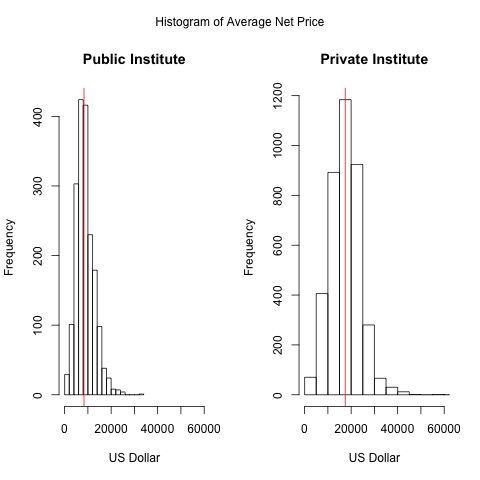
\includegraphics[width=150px]{../images/histogram-meanNetPrice} 

}




By comparing the 2 histograms, we can see that the simplified distribution of net price for public institutions is skewed-left, while net price of private colleges tends to follow a more normal-appearing distribution. \newline

The data reflects these differences by having stored many different net prices - average net price is categorized into different income quintiles for students. 

\begin{itemize}
\item USD 0 - 30,000
\item USD 30,001 - 48,000
\item USD 48,001 - 75,000
\item USD 75,001 - 110,000
\item USD 110,000+
\end{itemize}

Each quintile is further divided into 'Public' or 'Private'. 

\subsubsection{Standardized Test Scores}

Standardized Test Scores are an obvious piece of data that we could have students input into the Shiny App - weighing down schools they are substantially below the average for could definitely make a better model. This information is definitely more relevant to how likely a student may get admission rather than including as a positive metric of "quality" in the response variable. So, let's begin by looking at the general distribution of SAT and ACT scores.



{\centering 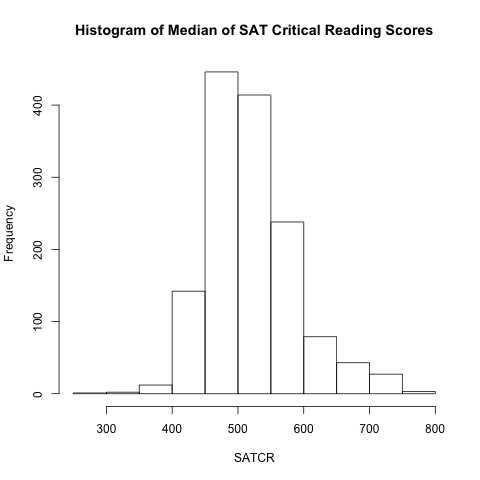
\includegraphics[width=150px]{../images/histogram-SATCRMedian} 

}


\begin{table}[ht]
\centering
\begin{tabular}{rrrrrrrrrr}
  \hline
 & Min. & Max. & Range & Median & 25th & 75th & IQR & Mean & SD \\ 
  \hline
1 & 298.00 & 757.25 & 459.25 & 511.50 & 475.50 & 556.25 & 80.75 & 520.90 & 66.81 \\ 
   \hline
\end{tabular}
\caption{Summary Statistics for SAT Critical Writing} 
\end{table}


From the histogram and the table above, we see that the median of SAT Critical Reading scores appears to have an approximately normal distribution, with the most frequent range of scores between 450 and 550. \newline

We could consider colleges with score higher than 556 to be outstanding (or, difficult to get in to) - but this would be a controversial, unfounded claim, so we mostly use the scores as metrics for the chances a student may or may not get in. Under considerable thought and some research, we decide to not weight up schools that have higher average test scores.



{\centering 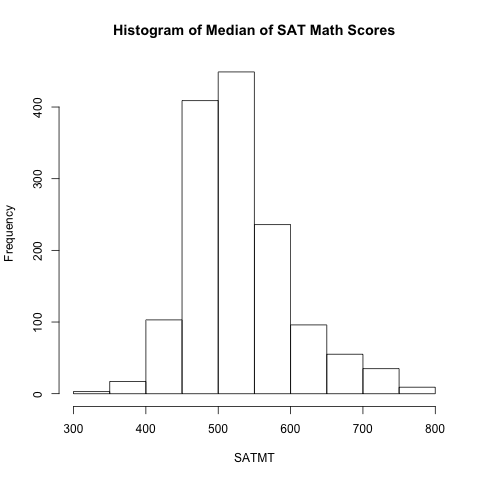
\includegraphics[width=150px]{../images/histogram-SATMTMedian} 

}


\begin{table}[ht]
\centering
\begin{tabular}{rrrrrrrrrr}
  \hline
 & Min. & Max. & Range & Median & 25th & 75th & IQR & Mean & SD \\ 
  \hline
1 & 305.00 & 783.75 & 478.75 & 516.00 & 482.31 & 563.17 & 80.86 & 528.66 & 70.38 \\ 
   \hline
\end{tabular}
\caption{Summary Statistics for SAT Math} 
\end{table}


The data for the math section of the SAT follows almost identical distribution to the Critical Reading, with the same most common range [450-550] and around a value of 553 for exceptionally difficult schools. We maintain the same decision as discussed above.\newline

Because a significant portion of colleges did not record or submit their SAT Writing scores to the original dataset, we don't analyze their distribution here.\newline

We may conduct similar analysis on reported ACT scores:



{\centering 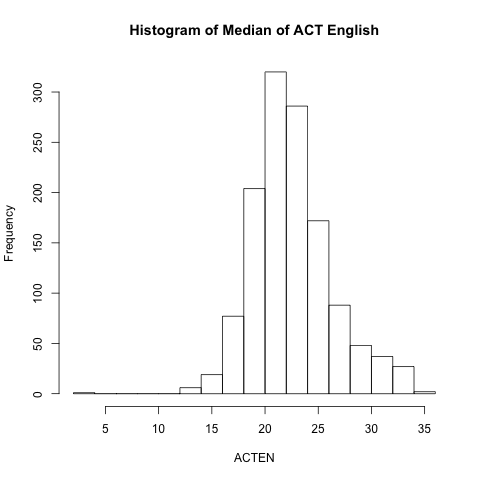
\includegraphics[width=150px]{../images/histogram-ACTENMedian} 

}


\begin{table}[ht]
\centering
\begin{tabular}{rrrrrrrrrr}
  \hline
 & Min. & Max. & Range & Median & 25th & 75th & IQR & Mean & SD \\ 
  \hline
1 & 2.00 & 34.40 & 32.40 & 22.17 & 20.16 & 24.60 & 4.44 & 22.69 & 3.78 \\ 
   \hline
\end{tabular}
\caption{Summary Statistics for ACT English} 
\end{table}


From the histogram and the table above, we can see that the median of ACT English scores basically follows a normal distribution, with most of the scores clustering between 20 and 24. We may consider colleges with such score higher than 24.6 to be exceptionally difficult to get in to.



{\centering 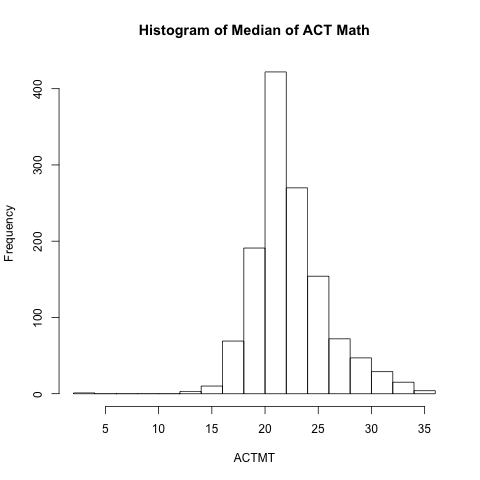
\includegraphics[width=150px]{../images/histogram-ACTMTMedian} 

}


\begin{table}[ht]
\centering
\begin{tabular}{rrrrrrrrrr}
  \hline
 & Min. & Max. & Range & Median & 25th & 75th & IQR & Mean & SD \\ 
  \hline
1 & 2.00 & 35.40 & 33.40 & 21.95 & 20.40 & 24.00 & 3.60 & 22.47 & 3.41 \\ 
   \hline
\end{tabular}
\caption{Summary Statistics for ACT Math} 
\end{table}



Lastly, we examine the ACT math distribution. We can see that the median of ACT Math scores basically follows a normal distribution, with most of the scores clustering between 20 and 24, and an average score higher than 24 appears to represent a school exceptionally difficult to attend.\newline

As discussed in the critical reading section, upon substantial thought, we decide that these scores may not be perfect, empirical markers of institutional quality, so we hesitate to include them in our baseline composite response metric. We do include scores, though, as an input that a student can manipulate. In our final app, if their score is lower than the average for that institution, the score for the school will be weighted down but still shown. This is not functionally equivalent to just including the average score in our response variable and weighting up schools that have higher ones, so we are much more satisfied with this method of including scores, as they definitely matter for college admissions. Thus, we are not suggesting that test scores are unimportant to the college process, but that they may not be great markers of objective quality. We include them only out of fairness to students, as recommending schools that they may not be qualified to apply to would be against our mission statement. We don't rule these schools out completely, instead, merely hesitating to immediately reccomend them, as they may have other statistics that make them strong potential schools, but out of reach of most applicants.\newline

Though this is representative of only a subsection of our research and exploratory analysis, we include this section as demonstration of our arduous process in determing what would be good to include in our model, both as part of our responsive "quality score" or as inputs for students, so they can be shown schools with student bodies more similar to who they are or schools that they could realistically get in to. Thus, this exploratory analysis was invaluable in getting a sense of some information about schools across the nation to inform our modeling decisions. \newline

To explain some actual decisions we made from this exploratory analysis, we decide to heavily include geographic location in determining output for students, as in-state tuition for public schools is more readily available in the dataset and out-of-state net price may not be as consistently available. Thus, if we wish to realistically model the net prices of public schools, we can only do so if the student is a resident of that state. This may be a minor shortcoming of our model, but it is a data limitation, not a creative one! Ethnicity of the student body in relation to a student's own is included in the model, as research indicates that attending a school with students of your racial/ethnic background can greatly improve comfort, success, retention, etc. Net price is obviously included in our response for obvious reasons - we can't, in good faith, recommend at-risk students to apply to schools with significantly higher net prices, as net price actually represents the \emph{final cost} of attendance after financial aid for each income bracket. Thus, it can included wholesomely and in good faith. Our last main piece of information analyzed, SAT/ACT scores, we decided were not worth including in our baseline model as quality indicators due to their imperfection. We begrudgingly but out of necessity include them as inputs for students that alter schools shown out of a desire to maintain an honest, truthful relationship with the students, showing them schools that are worth the application. Again, our mission is to create an interactive list of schools which are high-quality at a low-cost for students who need the help.

\maketitle
\section{Method}

In this section, we continue the discussion on how we decided upon the composite "quality" metric for high-quality, low-cost education for at-risk students. We later move on to their weighting and actual method implementation in the shiny app. \newline

One of the most common reasons students cite in choosing to go to college is the expansion of employment opportunities. This is of even greater intuitive importance to poorer students, who absolutely cannot afford to go to an expensive school that may leave them in permanent debt. To that end, data on the earnings and employment prospects of former students can provide key information. To measure the labor market outcome of individuals attending institutions of higher education, data on cohorts of federally aided students were linked with earnings data from de-identified tax records and reported back at the aggregate, institutional level. This dataset, however, is separate from the main College Scorecard dataset, and is included in a different .csv, \emph{Most-Recent-Cohorts-Treasury-Elements.csv} As mentioned earlier, although these datasets were separate at the start, we merge the two to allow for easy access to pertinent information that may only be contained in one of the datasets. Obvious data of interest only within this dataset are median earnings and median debt after graduation.\newline

So - we choose a set of columns that we feel, in aggregate, can represent in some small, objective measure, a school's quality - now, how do we actually create this score in practice? First, we standardize all of the included variables within their respective columns, then take z-scores, and use these z-scores in place of the actual values within each column. Thus, the average of any statistic will be given a score close to 0, with scores above given a more positive score, and scores below a more negative score. Then, we weight each metric with deliberation, experimentation, and consultation of literature. Importantly, some data points are actually desirable when substantially \emph{below} the average, such as net price or median debt, while others are obviously better if higher, such as median earnings or completion rate. Thus, we actually weight some pieces positively and other negatively in regards to the sign of their z-scores. Finally, these scores will alter and adjust both weighting and actual information as students enter and change their inputted answers. \newline

Eventually, we decided upon the following for our data included in the response and their weights:\newline



1 - Net Price, stratified by income. There are 5 income brackets within the dataset, so dependent upon which income bracket a student inputs, the score is recalculated to consider the relative z-score of their projected respective net cost of attendance. For students below a certain income level, we actually want to more heavily reward schools with very negative z-scores, as these schools, in totality, are anomalously cheap when compared to their counterparts. We decide that for lower income students, this is of more significant importance, as this is the net price of attending AFTER financial aid - and these are students who need to know exactly how much attending could cost. Thus, the columns the information is drawn from and the weights themselves are dynamically adjusted based on user input.

\begin{table}[ht]
\centering
\begin{tabular}{rlll}
  \hline
 & Variable & Weight & Condition \\ 
  \hline
1 & NetPrice & -0.05 & Default \\ 
  2 & NetPrice & -0.3 & Income in \$0-\$75,000 \\ 
  3 & NetPrice & 0.4 & Income in \$75,000+ \\ 
   \hline
\end{tabular}
\caption{Table of Net Price by conditional weights} 
\end{table}


2 - Repayment rate, split into 3 year repayment rate and 5 year repayment rate. To clarify, this column represents the proportion of students who have completely paid off their debt to the school after 3 and 5 years.  Specifically, we choose the columns of repayment rate by completers, as we do not wish to muddle the recommendation algorithm with students who are struggling to pay back their loans because they did not actually finish their education. While this could be interpreted as an oversight, we believe we are discussing college admissions with students who understand the hardships that getting a college education entails, and are willing to take the risk of attempting to complete. It would be unfair to their passion to attend to include the repayment rate for students who weren't able to finish - we presume that they are willing to take the risk and want to know the information pertaining to the goal they're trying to achieve, not what could happen. To eliminate variance, we include both the 3 year and the 5 year repayment rate at equal weighting in the final response quality metric.

\begin{table}[ht]
\centering
\begin{tabular}{rlll}
  \hline
 & Variable & Weight & Condition \\ 
  \hline
1 & 3 Year Repayment Rate & 0.1 & Default \\ 
  2 & 5 Year Repayment Rate & 0.1 & Default \\ 
   \hline
\end{tabular}
\caption{Table of Repayment Rate by weights} 
\end{table}



3 - Completion rate, in 150\% time (4+2 years) for all students at that particular institution. Of course, this is a loaded statistic, and although we briefly touched upon the discussion around which students are most likely to complete college and which are likely to not, we did brush over that the students we are working to accomodate are at-risk, and thus, are significantly more likely to struggle or possibly need to drop out. So, admittedly, this metric may be imperfect as it is not stratified to completion rate of students within specific income brackets. However, we believe it can still be appreciated and is important, perhaps indicative of some broader communal feeling at the school, and is worthy of inclusion. 

\begin{table}[ht]
\centering
\begin{tabular}{rlll}
  \hline
 & Variable & Weight & Condition \\ 
  \hline
1 & 4 Year Completion Rate & 0.7 & Default \\ 
   \hline
\end{tabular}
\caption{Table of Completion rate by weight} 
\end{table}


4 - Mean and median earnings, 10 years after beginning college. This is another imperfect statistic to include, as to study earnings 6 years (in theory) after graduation, we must use data from students who started college 10 years ago, which is outside of the framework of our data set. However, because it is contemporary information and is often referred to as a significant and crucial piece of measuring a more objective sense of monetary quality of university attendance, we include it despite its flaws. We use both the mean and median earnings 10 years after beginning, again, to reduce variance and to legitimize claims of a potential expectation of salary in the future. While this may not be why every student attends college, it is important to a large number of students and a good indicator of the capability for social mobility provided by an institution - which is exactly what we seek to measure and return.

\begin{table}[ht]
\centering
\begin{tabular}{rlll}
  \hline
 & Variable & Weight & Condition \\ 
  \hline
1 & 10 Year Mean Earnings & 0.7 & Default \\ 
  2 & 10 Year Median Earnings & 0.7 & Default \\ 
   \hline
\end{tabular}
\caption{Table of Mean/Median Earnings by weights} 
\end{table}


5 - Percentage of the student body which has/could have a Pell Grant. This is a metric entirely new to us, but is discussed extensively in educational literature as a prescient indicator of built-in, intentional, positive institutional affordances to low-income students. The Pell Grant is a federal loan given to extremely low income students to allow for their attending college with very little to begin with. Thus, scholars reason that schools who integrate into their agenda encouragement and enabling of Pell Grant student attendance may have more amorphous, hard-to-capture support systems in place as well which could allow these students to succeed. In short, they reason that if a school intentionally lets in a bunch of kids with Pell Grants, they'll have programs specifically tailored to those kids to do well. This is a very positive indicator for at-risk, low-income, minority students, so we include it. To allow for students of all income brackets to use our score generator, though, we only include the Pell Grant percentage for students in lower income brackets, and ignore it for students who do not fit a reasonably similar criterion. \newline

Additionally, the existence of a community of people similar to you at a school is vitally important to success, and if a school has a high number of Pell Grant students, it may reduce the shame or uncomfortability that stems from being from a household of very low income - being around people who have come from similar hardships to you has proven time and time again to help in dramatic ways.  

\begin{table}[ht]
\centering
\begin{tabular}{rlll}
  \hline
 & Variable & Weight & Condition \\ 
  \hline
1 & Pell Grant & 0.1 & Default \\ 
  2 & Pell Grant & 0.5 & Income in \$0-\$30,000 \\ 
   \hline
\end{tabular}
\caption{Table of Pell Grant Percentage by conditional weights} 
\end{table}


6 - Median debt after attending. This is another statistic that is very difficult to generalize out to all students, but we incldue it anyway as it is of obvious relevance, regardless of equal applicability to all students. This is a very real, concrete number and even if it is unfair to create a median debt over the entire student body, it seems to have some legitimacy when compared to other schools. If a school has a higher median debt, for example, this could either be an indicator of a lack of substantial financial aid afforded to students, or, more interestingly, suggestive of a student body which is generally lower-middle class - able to sort-of afford attendance, not of low enough income to get substantial financial aid, not of high enough income to have no debt at all. Educational scholars also suggest that it is important to include, so we do so, and it plays a minor role in our final composite metric.

\begin{table}[ht]
\centering
\begin{tabular}{rlll}
  \hline
 & Variable & Weight & Condition \\ 
  \hline
1 & Median Debt & -0.1 & Default \\ 
   \hline
\end{tabular}
\caption{Table of Median debt by weight} 
\end{table}


7 - First generation student percentage. This is included for very similar reasons to the Pell Grant percentage - if an institution is willing to take on a large number of students, they likely have programs in place to accomodate them. It also suggests that a school will have many other first generation students who would be able to provide a support network. Like the Pell Grant percentage, we only include the variable if a student indicates that they are a first-generation student. We believe that having such a choice for the users would be considerate. They have the freedom to negate it as well.

\begin{table}[ht]
\centering
\begin{tabular}{rlll}
  \hline
 & Variable & Weight & Condition \\ 
  \hline
1 & First Generation & 0 & Default \\ 
  2 & First Generation & 0.2 & First Generation \\ 
   \hline
\end{tabular}
\caption{Table of First Generation percentage by conditional weights} 
\end{table}


8 - Intended field of study. During the iterative process of creating this app, we ran into issues with weighting and variable inclusion. At one point, our app only recommended art schools, partially due to errors in weighting and partialy due to a lack of narrowing the application field by limiting the search to schools which actually had some semblance of a program you were interested in. Thus, we boost a college's score if it offers the program that the student is interested in, without discounting other good schools which may not exactly offer that major.

\begin{table}[ht]
\centering
\begin{tabular}{rlll}
  \hline
 & Variable & Weight & Condition \\ 
  \hline
1 & Major & 0.1 & Default \\ 
  2 & Major & 0.3 & Selected major \\ 
   \hline
\end{tabular}
\caption{Table of Field of study by conditional weights} 
\end{table}


9 - Similar Ethnicity percentage. As discussed in previous segments, a school which has real communities of students of many backgrounds and diverse origins is important to both the quality of the school but also to minority students who may want to be near people of the same Ethnicity. This is a simple metric, and is only weighted upon the ethnicity that a student says they are a member of. Thus, if I enter that I am a black student, it will use the z-scores of the percentage of the student body that is black and dynamically alter the weights to favor schools which have higher percentages of black students. Again, having sizable minority percentages may also imply that the school has other affordances to at-risk students who may need the help.

\begin{table}[ht]
\centering
\begin{tabular}{rlll}
  \hline
 & Variable & Weight & Condition \\ 
  \hline
1 & Ethnicity & 0 & Default \\ 
  2 & Ethnicity & 0.1 & Selected ethnicity \\ 
   \hline
\end{tabular}
\caption{Table of Ethnicity Percentage by conditional weights} 
\end{table}


10 - Test Scores. While we only begrudgingly include this piece in a minor way, it is admittedly still important to not reccomend students schools which are substially out of their reach via a large test score mismatch. While we're dubious of its status as actually an indicator of quality in any way, pragmatically, schools do have cutoffs on scores and we don't want these at-risk students to waste their time applying to programs they may have no chance of being accepted to. However, as we don't want to rule out any schools completely, we only slightly weight up a school if it fits the entered score threshold.

\begin{table}[ht]
\centering
\begin{tabular}{rlll}
  \hline
 & Variable & Weight & Condition \\ 
  \hline
1 & Test Score & 0 & Default \\ 
  2 & Test Score & 0.1 & Input test score \\ 
   \hline
\end{tabular}
\caption{Table of Standardized Test Scores by conditional weights} 
\end{table}


Thus, we arrive at our 10-section composite metric of school "quality", which is especially geared towards at-risk, low-income, minority students, but can be adjusted to fit any student's needs reasonably well. We chose these criterion based upon deliberation, experimentation, and research. 
\maketitle
\section{The App // Results}


Now that we've established the composite quality score metric, we can talk in more detail about the actual app itself and what the student inputs. First, they are met with a small introduction which lays out the purpose of the app that we have reiterated over and over - providing a low-cost, high-quality education to students who need it. Then, the student enters in their:
\begin{itemize}
\item State of residence
\item Ethnicity
\item Income bracket
\item First Generation Status
\item Intended Field of Study
\item SAT/ACT scores
\end{itemize}

As discussed at length in the methods section, all of these were deemed as relevant to determining the dynamic aspects of the response score - the remaining factors, of median debt, repayment rate, and completion rate, are all constant across the university and not stratified in any way, so they cannot react to user input. However, besides these 3 flat response values, the remaining 7 pieces of the composite score metric are all dynamic and change both weight and information itself based on user input.\newline

They also see a complete map of all institutions in the U.S., and when they select a state, another map will zoom in on their particular state and show a resized map of regional schools.\newline

So, we've established what the student enters and what they see. We then return a list of the top 10 matching schools, ordered on our composite quality metric, which best fit their portfolio of inputs and information. The top matching school will always have a 100 score value, and the remaining scores are computed proportionately from this arbitrary top scoring institution. To gather more information about schools a user is interested in, they can copy/paste the ID of a particular school into the box on the left, which pulls up more detailed summary statistics for the student to interpret, such as projected net price of attendance (after financial aid), percent of students of their ethnicity, percent of students within their major, and a standardized test score spread. While this is in no way exhaustive or comprehensive, we believe that the computed score will be of great value to potential applicants, as it will offer schools which empirically meet their demands but that they may not have heard of or searched for without the intervention of our analytic process. 

\maketitle
\section{Conclusions}

We began with a massive primary source data set from \emph{College Scorecard}, spread over different years, with major swaths of relevant data not even included. We considered what we'd find meaningful to do, and decided an app helping at-risk, low-income, minority students under the guise of providing a consulting service to an NGO would be both interesting and gratifying. We then carried out extensive data cleaning, exploratory analysis, reading, experimentation, and research to figure out what we could actually do with this data. We decided that an app which returns schools that would serve students who need education but  may not know about was a poignant direction to go. After substantial deliberation, we decided upon creating an ad-hoc, composite "school quality metric" that would serve to sort a list of outputted colleges to students who interact with the app. This was compiled together with substantial thought and work, and the weighting and inclusion of variables is extremely fine-tuned and the result of many careful considerations. The final app, which students interact with and input values to was also the product of endless deliberation - what was relevant to include, what was unnecessary, what to show, how to sort, etc. In the end, we are happy with our final app and the composite "school quality metric" which we composed. The dynamic, interactive nature of the metric is a source of great pride for all of us in the group, and we hope that it will return schools that students would not have thought of but would truly give them what any student wants, in the end, customized to their specific situation and intentions: a high-quality, low-cost education.\newline

Thank you for reading and we hope the app serves you well.\newline

From all of us at the consultant team,

\textit{- Liang Hao, Bret Hart, Andrew Shibata, and Gary Nguyen}


\end{document}
